\documentclass{article}
\usepackage[hyphens]{url}
\usepackage{mathtools}
\usepackage{amsmath}
\usepackage{listings}
\usepackage{graphicx}
\usepackage[margin=1in]{geometry}
\usepackage{float}
\floatstyle{boxed}
\restylefloat{figure}
\lstset{basicstyle=\footnotesize, breaklines=true}
\begin{document}


\title{CS595 Intro to Web Science, Assignment \#6}
\author{Valentina Neblitt-Jones}
\date{October 31, 2013}
\maketitle



\section*{Question 1}

We know the result of the Karate Club (Zachary, 1977) split. Prove or disprove that the result of split could have been predicted by the weighted graph of social interactions. How well does the mathematical model represent reality? \\

Generously support your answer with all supporting equations, code, graphs, arguments, etc. \\

Useful sources include:  \\

\begin{itemize}
\item Original paper
	\begin{itemize}
	\item \url{http://aris.ss.uci.edu/~lin/76.pdf}
	\end{itemize}
\item Slides 
	\begin{itemize}
	\item \url{http://www-personal.umich.edu/~ladamic/courses/networks/si614w06/ppt/lecture18.ppt}
	\item \url{http://clair.si.umich.edu/si767/papers/Week03/Community/CommunityDetection.pptx}
	\end{itemize}
\item{Code and data}
	\begin{itemize}
	\item \url{http://networkx.github.io/documentation/latest/examples/graph/karate_club.html}
	\item \url{http://nbviewer.ipython.org/url/courses.cit.cornell.edu/info6010/resources/11notes.ipynb}
	\item \url{http://stackoverflow.com/questions/9471906/what-are-the-differences-between-community-detection-algorithms-in-igraph/9478989#9478989}
	\item \url{http://stackoverflow.com/questions/5822265/are-there-implementations-of-algorithms-for-community-detection-in-graphs}
	\item \url{http://konect.uni-koblenz.de/networks/ucidata-zachary}
	\item \url{http://vlado.fmf.uni-lj.si/pub/networks/data/ucinet/ucidata.htm#zachary}
	\end{itemize}
\end{itemize}
\subsection*{Answer to Question 1}

It was difficult to decide on approach here since we were provided information both on R and Python. Initially I thought Python followed by R for the graphs which appear to be expected due to the mention of graphs in the question. I started trying to follow the example and it was clear my computer was missing some important software. However, attempt to rectify that failed in more areas than one. After Corren McCoy raised the issue of getting the data set into R, it seemed that R was a possibility for answering this question. Scott Ainsworth's earlier lecture on R did reveal much more capability than we had employed on the previous assignment which had Python doing most of the heavy lifting and a smaller amount of work using R to create the graphs. Although Shawn Jones and I have had different approaches to previous problems, we were in the same boat this time as far as doubts about tools to use for this problem. We both experimented with edge.betweenness.community, fastgreedy.community, walktrap.community, spinglass.community, leading.eigenvector.community, label.propagation.community and I even tried infomap. We were not finding what we expected. Then Corren provided her steps in using R to the class email list.

%\begin{enumerate}
%\item edge.betweenness.community to find the shortest path among "all" edges
%\item Iterated over the generated graph to recalculate the edge weights
%\item Sorted the edges and remove the one with the highest weight
%\item As the loop condition, check whether all the edges were examined or the graph had the desired number of clusters
%\item When it reaches two communities, plot the graph.
%\end{enumerate}

First I imported the karate club data. Then I assigned it to ``k'' and plotted the graph. Then I calculated the edge betweenness of k. Next I ordered the result in decreasing order. The next thing to figure out was how to reference an item in order to remove it. I did a search for this and shared a Stack Overflow page with Shawn. The first answer was not quite right, but he found something of value lower on the answer page. Negative indices means do not include the element. So we used -1 to pop the element off the front. Next ``get.edge'' expects the graph name (k) and the id (a) and returns the end points of the edge with the edge id supplied and ``delete.edges'' removes the specified edge from the graph and preserves the vertices. P is used to select edges based on their end points. Then I plotted the graph again in order to track the graph changes. This repeats until the number of clusters is equal to two. (Listing \ref{code})

\begin{lstlisting}[frame=single, caption=karateClub.R, label=code]
data(karate)
k <- karate
plot.igraph(k) #Original graph

repeat
	{
	kedge <- edge.betweenness(k)
	korder <- order(kedge, decreasing=TRUE)
	a <- korder[-1]
	b <- get.edge(k,a)
	k <- delete.edges(k, E(k,P=b))
	plot.igraph(k)
	if (clusters(k)$no == 2) break()
	}
\end{lstlisting}

\begin{figure}[H]
\centering
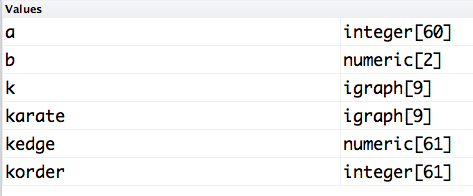
\includegraphics[scale=0.50]{q1/types}
\caption{Results of Assignments}
\label{types}
\end{figure}

%\begin{figure}[H]
%\centering
%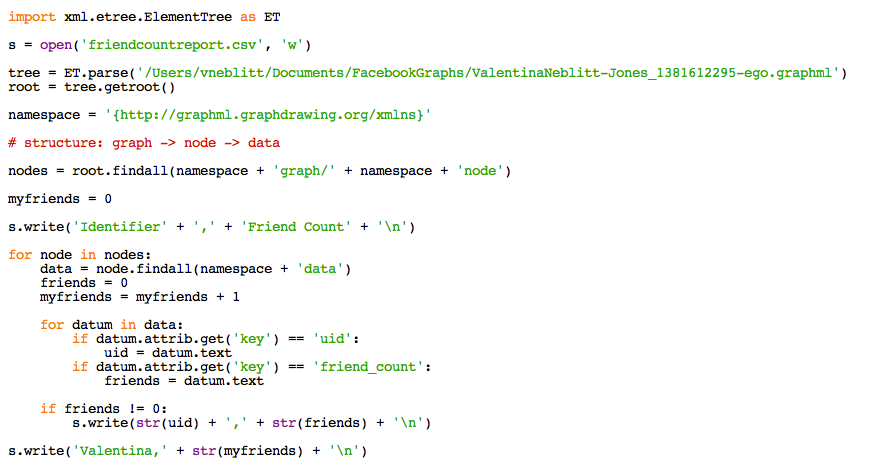
\includegraphics[scale=0.50]{q1/GetFriendCountsCode}
%\caption{Showing Friend Count}
%\label{GetFriendCountsCode}
%\end{figure}

\begin{figure}[H]
\centering
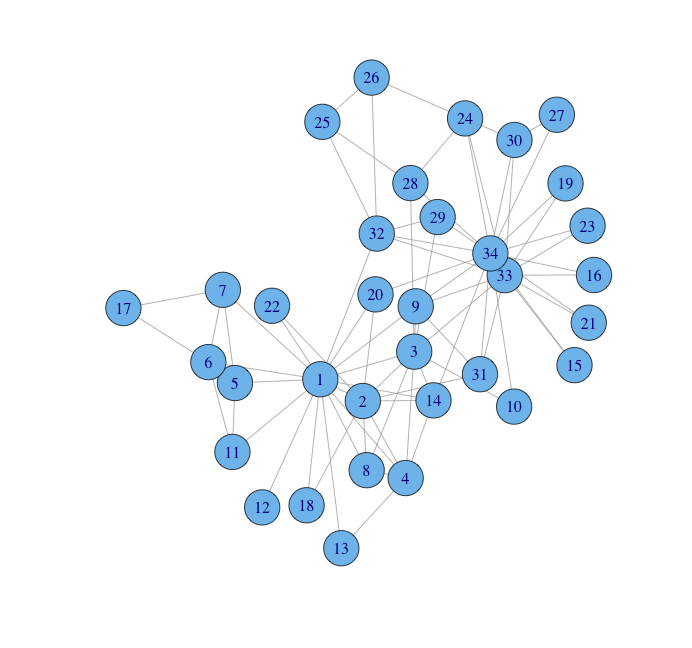
\includegraphics[scale=0.50]{q1/original}
\caption{Before Community Split}
\label{before}
\end{figure}

\begin{figure}[H]
\centering
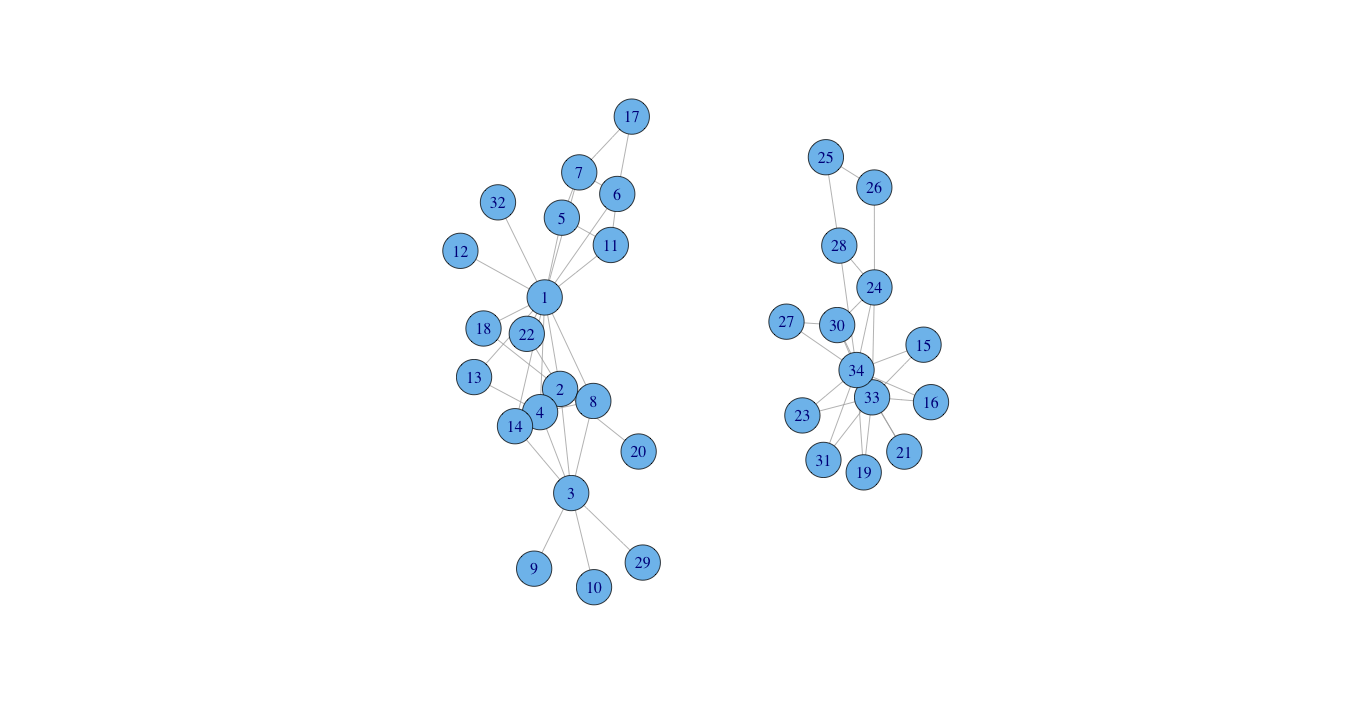
\includegraphics[scale=0.50]{q1/step18}
\caption{After Community Split}
\label{after}
\end{figure}



\begin{table}[!h]
\centering

\begin{tabular}{c c c c}
\hline
Identifier & Model &  Actual & Hit/Miss \\
\hline
\hline
1 & Mr. Hi & Mr. Hi & Hit \\
2 & Mr. Hi & Mr. Hi & Hit \\
3 & Mr. Hi & Mr. Hi & Hit \\
4 & Mr. Hi & Mr. Hi & Hit \\
5 & Mr. Hi & Mr. Hi & Hit \\
6 & Mr. Hi & Mr. Hi & Hit \\
7 & Mr. Hi & Mr. Hi & Hit \\
8 & Mr. Hi & Mr. Hi & Hit \\
9 & Mr. Hi & Mr. Hi & Hit \\
10 & Mr. Hi & John & Miss \\
11 & Mr. Hi & Mr. Hi & Hit \\
12 & Mr. Hi & Mr. Hi & Hit \\
13 & Mr. Hi & Mr. Hi & Hit \\
14 & Mr. Hi & Mr. Hi & Hit \\
15 & John & John & Hit \\
16 & John & John & Hit \\
17 & Mr. Hi & Mr. Hi & Hit \\
18 & Mr. Hi & Mr. Hi & Hit \\
19 & John & John & Hit \\
20 & Mr. Hi & Mr. Hi & Hit \\
21 & John & John & Hit \\
22 & Mr. Hi & Mr. Hi & Hit \\
23 & John & John & Hit \\
24 & John & John & Hit \\
25 & John & John & Hit \\
26 & John & John & Hit \\
27 & John & John & Hit \\
28 & John & John & Hit \\
29 & John & John & Hit \\
30 & John & John & Hit \\
31 & John & John & Hit \\
32 & Mr. Hi & John & Miss \\
33 & John & John & Hit \\
34 & John & John & Hit \\
\hline
\end{tabular}
\caption{Results of Model vs. Actual}
\label{hitsmisses}
\end{table}

The resulting graph (Figure \ref{after}) supplies the information for the Model column in Table \ref{hitsmisses} and reveals that there are 32 hits, 2 misses or 94\% hits, 6\% misses. This is close to the paper's results - 33 hits, 1 miss or 97\% hits, 3\% misses. So the model is close to representing reality.\\

\newpage

\section*{Extra Credit, 3 Points}

We know the group split into two different groups. Suppose the disagreements in the group were more nuanced -- what would the clubs look like if they split into groups of 3, 4, and 5?

%\begin{table}[!h]
%\centering
%\caption{Results of Model vs. Actual}
%\begin{tabular}{c c c c}
%\hline
%Identifier & Model &  Actual & Hit/Miss \\
%\hline
%\hline
%0.150 & 0.014 & Mr. Hi & Hit \\
%0.085 & John & Mr. Hi & Hit \\
%\hline
%\end{tabular}
%\end{table}

\subsection*{Answer to Extra Credit}

Working with the assumption that the solution to the regular question is correct, I just changed the cluster number in Listing \ref{code} to match 3, 4 and 5 separately. With more factions the larger clusters still belong to Mr. Hi and John. Clusters not including them are quite small. In all three cases, factions without Mr. Hi or John are of size four. In all three cases, factions containing Mr. Hi are bigger than those containing John. Table \ref{compares} shows the counts for each clusters. Figure \ref{after3} has one size 4 cluster. Figure \ref{after4} has two size 4 clusters. Figure \ref{after5} has three size 4 clusters. 

\begin{figure}[H]
\centering
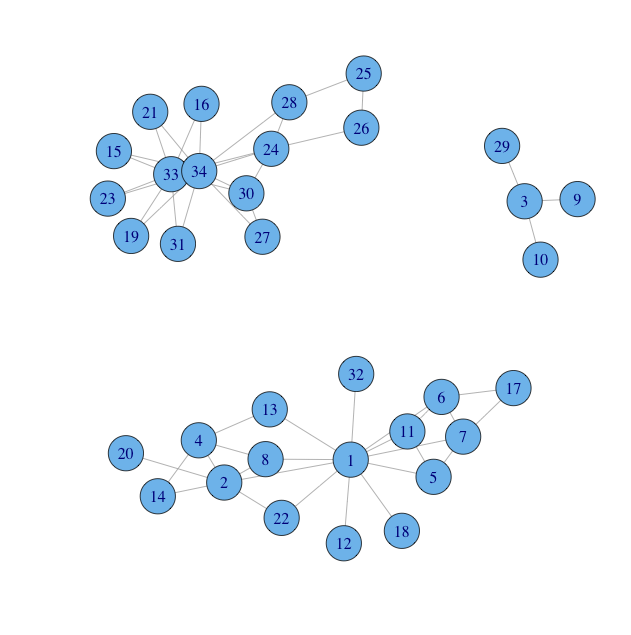
\includegraphics[scale=0.50]{ec/karateclub3}
\caption{Karate Club with Three Factions}
\label{after3}
\end{figure}

\begin{figure}[H]
\centering
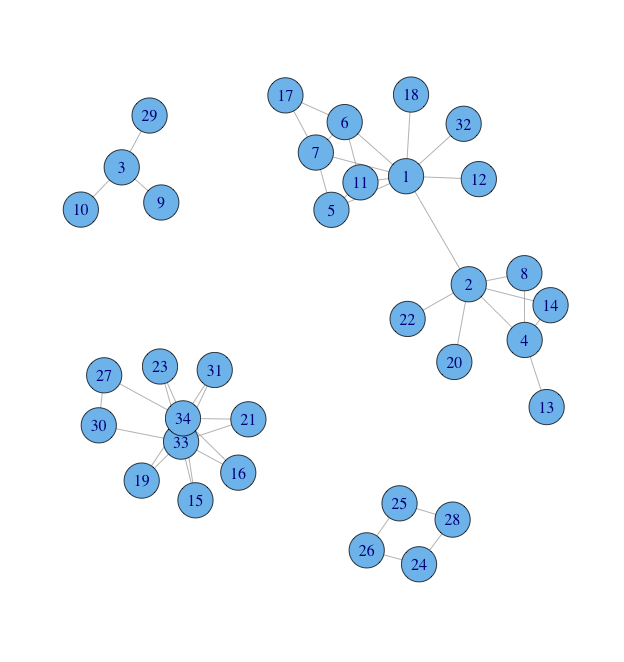
\includegraphics[scale=0.50]{ec/karateclub4}
\caption{Karate Club with Four Factions}
\label{after4}
\end{figure}

\begin{figure}[H]
\centering
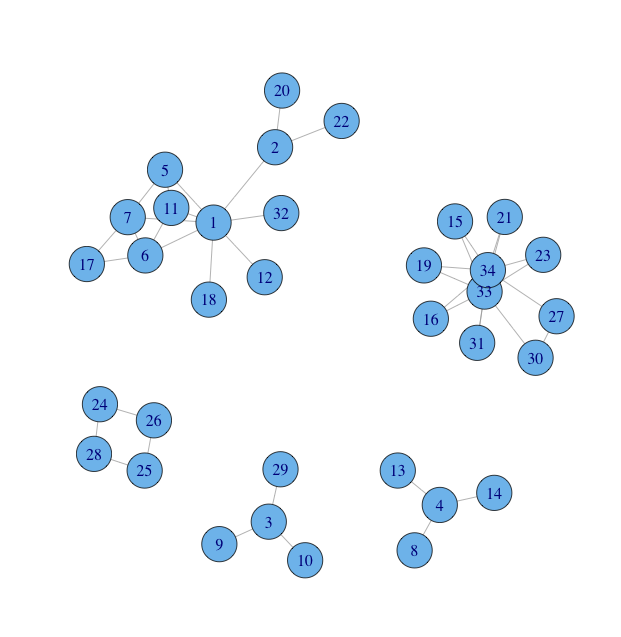
\includegraphics[scale=0.50]{ec/karateclub5}
\caption{Karate Club with Five Factions}
\label{after5}
\end{figure}

\begin{table}[!h]
\centering

\begin{tabular}{c c c c}
\hline
Clusters & Mr. Hi &  John & Others \\
\hline
\hline
3 & 16 & 14 & 4  \\
4 & 16 & 10 & 4  \\
5 & 12 & 10 & 4  \\
\hline
\end{tabular}
\caption{Comparison of Three Different Cluster Sizes}
\label{compares}
\end{table}


\newpage

\section*{Resources}

\begin{itemize}
\item Csardi, Gabor. Gaining information about graph structure. \url{http://igraph.sourceforge.net/doc/R/structure.info.html}
\item Csardi, Gabor. Method for structural manipulation of graphs. \url{http://igraph.sourceforge.net/doc/R/graph.structure.html}
\item Csardi, Gabor. Network Analysis and Visualization. \url{http://igraph.sourceforge.net/doc/R/00Index.html}
\item Csardi, Gabor. Network Analysis with igraph. \url{http://igraph.sourceforge.net/igraphbook/index.html}
\item Csardi, Gabor. Vertex and edge sequences and iterators. \url{http://igraph.sourceforge.net/doc/R/iterators.html}
\item Poulson, Barton. R Statistics Essential Training. \url{http://www.lynda.com/course20/R-tutorials/R-Statistics-Essential-Training/142447-2.html}
\item Rice, Ken \& Lumley Thomas. Writing Loops. \url{http://faculty.washington.edu/kenrice/sisg/SISG-08-05.pdf}
\item Stack Overflow. Are there implentations of algorithms for community detection in graphs? \url{http://stackoverflow.com/questions/5822265/are-there-implementations-of-algorithms-for-community-detection-in-graphs}
\item Stack Overflow. How can I remove an element from a list \url{http://stackoverflow.com/questions/9998667/r-syntax-for-selecting-all-but-two-first-rows-in}
\item Stack Overflow. What are the differences between community detection algorithms in igraph? \url{http://stackoverflow.com/questions/9471906/what-are-the-differences-between-community-detection-algorithms-in-igraph/9478989#9478989}
\item Zachary, Wayne. An Information Flow Model for Conflict and Fission in Small Groups. \url{http://aris.ss.uci.edu/~lin/76.pdf}


\end{itemize}

\end{document}